\chapter{Ordinary Differential Equations III: Eigenvalue Problems}\label{ch:ode3}

Another important mathematical problem involving differential equation is the eigenvalue problem. In general it is a linear differential equation:
\begin{equation}\label{eq:eigen_equation}
\mathcal{L} y = \lambda y
\end{equation}
where $\mathcal{L}$ is a linear operator and $\lambda$.  We want to find \emph{eigenvalues} $\lambda$ and corresponding \emph{eigenfunctions} $y$. This equation is homogeneous and thus the magnitude of $y$ cannot be determined.  If $y(x)$ is a solution, then $c y(x)$ is also a solution where $c$ is any constant.  We utilize this property in the numerical methods.

A linear operator popular in physics has a form
\begin{equation}\label{eq:linear_operator}
\mathcal{L} = a \dv[2]{x} + p(x) \dv{x} + q(x)
\end{equation}
where $a$ is a constant, and the functions $p(x)$ and $q(x)$ do not depend on $\lambda$ nor $y$.   Explicitly writing \eqref{eq:eigen_equation}, we obtain an ODE
\begin{equation}
a y'' + p(x) y' + q(x) y = \lambda y\,.
\end{equation}
In this chapter we focus on this operator. 

Eigenvalue problems are different from the regular boundary value problems we investigated in the previous chapter. 
First of all, the value of $\lambda$ is not known. In general, $y(x)$ depends on $\lambda$ and we must determine both  $\lambda$ and $y(x)$ simultaneously.  How can we do that?  Suppose we use an arbitrary value for $\lambda$ and solve the ODE.  Let us write the solution as $y(x;\lambda)$ . The solution must satisfies boundary condition $y(x_\textsc{L};\lambda)=y_\textsc{L}$ and $y(x_\textsc{R};\lambda)=y_\textsc{R}$.  It looks that we can find the eigenvalue $\lambda$ by a root finding method.  However there are two equations to satisfy with a single parameter$\lambda$, which is not possible in general. The solution exists only for $y_\textsc{L}=y_\textsc{R}=0$.\cite{homogeneous_bvp1,homogeneous_bvp2} or the periodical boundary condition $y(x+L)=y(x)$.  

Second difference is that there can be many different solutions, which we write as
$\lambda_i, (i=1, 2, \cdots, N)$ and the corresponding eigenfunctions $y_i(x)$. In many cases, there are infinitely many solutions ($N=\infty$).
Some applications want to know one specific solution, usually the one with the smallest (or largest) eigenvalue.  Other applications want to know multiple solutions. It is hard for a numerical method to find all of them.  
Further complication arises when two different solutions have the same eigenvalue (degeneracy).  We do not discuss degeneracy in this chapter.

Apart from these differences, the numerical methods to solve the boundary value problems in the previous chapter still can be used to solve the eigenvalue problems. In this chapter, we focus on the shooting method.   There are other methods. Lowest eigenvalues can be obtained by numerical minimization of functionals, which we discuss in Chapter 8. We can convert eigenvalue problems to initial value problems of partial differential equations, which will appear in Chapter 13.  Yet, there is another method based on stochastic dynamics (diffusion Monte Carlo simulation), which will be introduced in Chapter 18.

Eigenvalue problems in matrix form are also common in physics, particularly in quantum mechanics where $\mathcal{L}$ is a square matrix and $y$ is a column vector.  Mathematically speaking, the matrix version is essentially the same as the present one.  In fact, we can convert a differential equation form of an eigenvalue problem to a matrix form using a basis set.  We will discuss the matrix version in Chapter 10.

\noindent
\section{Shooting Method for Eigenvalue Problems}

The basic idea is exactly the same as the shooting method in Chapter 5.  We guess a value of $\lambda$ and shoot. Change the value  and shoot again until we hit the target.  The target is one of the boundary condition.  Given $lambda$, we integrate the ODE from one of the boundaries, say $x_\textsc{L}$, using a numerical method such as the Numerov method.  The solution is a function of $\lambda$ which we write as $y(x;\lambda)$.  The boundary condition at $x_\textsc{L}$ is automatically satisfied when the ODE is solved numerically.   However, the other boundary condition at $x_\textsc{R}$ is not automatically satisfied. Only correct values of $\lambda$ can satisfy both boundary conditions. Therefore, we need to look for $\lambda$ that satisfies the other boundary condition, $y(x_\textsc{R},\lambda)=0$. This is just a root finding problem.  We adjust the value of $\lambda$ until the boundary conditions are satisfied.  

There is another way to satisfy the both boundary conditions. Integrate the ODE from both ends $x_\textsc{L}$ to some mid point $x_\textsc{C}$ and also backward from and $x_\textsc{R}$  to $x_\textsc{C}$. Then, we have two solution,  forward solution $y_+(x)$ for $x_\textsc{L}<x<x_\textsc{C}$ and backward solution $y_-(x)$ for $x_\textsc{C}<x<x_\textsc{R}$.  We can match these two solutions at $x_\textsc{C}$ by adjusting  their scale.  However, they do not connect smoothly at $x_\textsc{C}$ unless we have correct value for $\lambda$.  In this case, the root finding process solves $y_-^\prime(x_\textsc{C})=y_+^\prime(x_\textsc{C})$. We change $\lambda$ until this condition is satisfied.  This approach has an advantage in some case, particularly if the system has a useful symmetry such as parity.

A problem of the shooting method is that we don't know which eigenvalue we will find.  The secant method does not guarantee the eigenvalue nearest to the initial guess. If we want to find a specific eigenvalue, the bisection method is better if the target eigenvalue is bracketed. 

\bigskip 
\begin{myalgobox}
   \Algorithm{Shooting method with secant root finding}\label{algo:eigen_shooting_secant}
   \begin{minipage}{5.5in}
      \begin{enumerate}
         \item Guess a value of eigenvalue $\lambda_1$.  The subscript "1" indicates the first try.
         \item Starting with a boundary value $y(a)=0$.
         \item Assign a value to the next point $y(a+h)$.  Any value is OK since the magnitude is arbitrary.
         \item Integrate the ODE using a numerical method to the other end and get the value of $y_1=y(b)$.  This is the first output.
         \item If $|y_1| < \text{tolerance}$ then we find a solution. Otherwise continue to next step.
         \item Guess a new value of eigenvalue $\lambda_2$.  This is the second try.
         \item Integrate the ODE in the same way as step 4 and get the new value for $y_2=y(b)$.  This is the second output.
         \item If $|y_2| < \text{tolerance}$ then we find a solution. Otherwise continue to next step.
         \item Now, we enter a loop of the secant method.
         \item $\lambda_{n+1} = \lambda_{n} - \displaystyle\frac{\lambda_{n} - \lambda_{n-1}}{y_{n}-y_{n-1}} y_{n}$.  Here, the $(n+1)$-th try is suggested by the secant method.
         \item Solve the Newton equation with $\lambda_{n+1}$ as initial condition and get $y_{n+1} = y(b)$.
         \item If $|y_{n+1}| < \text{tolerance}$ then we find a solution.  Otherwise repeat from step 10.
      \end{enumerate}
   \end{minipage}
\end{myalgobox}

\bigskip
\begin{example}[Eigen modes of standing waves]\label{eq:eigen_modes}
	A standing wave in a stretched string is a simplest eigenvalue problem.  The vertical displacement of the string $y(x)$ at position $x$ is determined by the folowing eigen value equation:
	\begin{equation}\label{eq:eigen_modes}
	   \dv[2]{y}{x} = \lambda y
	\end{equation}
	with boundary conditions $y(0)=y(1)=0$.  The exact answer is well known. The eigenvalue is $\lambda_n = - (n \pi)^2$ and the corresponding eigenfunction  $y_n(x) = A \sin (n \pi  x)$ where $n$ is any non-negative integer and $A$ is any non-zero constant.
	Program \ref{prog:standing_wave} solves this problem using Algorithm \ref{algo:eigen_shooting_secant}.  Figure \ref{fig:shooting} illustrates the simple idea of shooting method.  When $\lambda=-9$, the solution overshoots the target boundary.  On the other hand, when $\lambda = -11$, the solution undershoot and misses the target again.  A certain value of $\lambda$ between the two values, the trajectory must hit the target.  That is the eigenvalue.  The program finds $\lambda=-9.869044$ which is in good agreement with the exact value $\lambda_\text{exact} = - \pi^2=-9.8696044$.
	
	\bigskip
	\exercise Solve the same problem with the bisection method (Algorithm \ref{algo:eigen_shooting_secant}).
	
   \vfill
   
\end{example}

	\begin{figure}[tb]
		\centering
		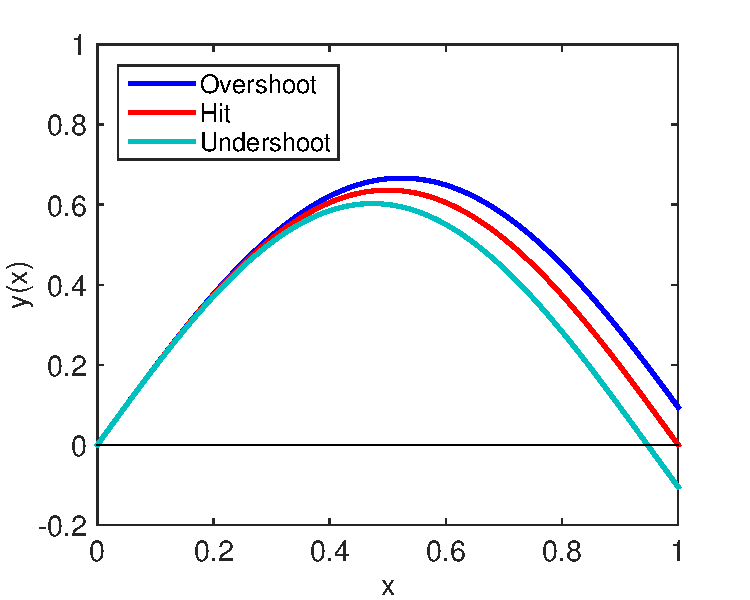
\includegraphics[width=2.5in]{07.ode3/shooting.pdf}
		\caption{Illustration of the shooting method. Equation (\ref{eq:eigen_modes}) is integrated with three different values of $\lambda$.  When $\lambda=-9$ (blue) , the solution overshoots the target boundary.  On the other hand, when $\lambda = -11$ (turquoise), the solution undershoots it. Therefore, the correct answer should be between the two values. When $\lambda=-9.8696044$ (red), the solution hits the target and thus it is the eigenvalue.}
		\label{fig:shooting}
	\end{figure}
	

	
	\bigskip


%\noindent
%\section{Periodic Boundary Conditions}
%
%To be written.



\noindent
\section{Applications in Physical Problems}



\subsection{Quamtum Harmonic Oscillator}\label{sec:qmho_eigenvalue}


Energy eigenvalues of a harmonic oscillator are determined by 
\begin{equation}\label{eq:qmho_eigenvalue}
\left [-\frac{\hbar^2}{2m} \frac{\md^2}{\md x^2} + \frac{m \omega^2 x^2}{2} \right ] \psi (x) = E \psi(x)
\end{equation}
where $m$ and $\omega$ are the mass and frequency of the oscillator, respectively.\cite{qmho} We want to determine eigenvaue $E$ and eigenfunction $\psi(x)$.  The boundary condition is $\displaystyle\lim_{|x| \rightarrow \infty} \psi(x) = 0$.  As usual, we replace this boundary condition with $\psi(\pm L) = 0$ where $L$ is a sufficiently large but finite quantity. Changing the units of length and energy as $\xi = \sqrt{\displaystyle\frac{m \omega}{\hbar}} x$ and energy $\lambda = \displaystyle\frac{2 E}{\hbar\omega}$, the above equation is simplified to\cite{qmho}
\begin{equation}\label{eq:qmho_eigen_simple}
\left [ \frac{\md^2}{\md \xi^2} - (\xi^2 - \lambda) \right ] \psi(\xi) = 0.
\end{equation}
which is suitable for the Numerov integration.
The exact solution is well known: $\lambda_n = 2 n + 1,\, n=0, 1, \cdots$ and corresponding eigenfunctions are given by
\begin{equation}
\psi_n(\xi) = \frac{1}{\sqrt{2^n n! \sqrt{\pi}}} \me^{-\xi^2/2} H_n(\xi)
\end{equation}
where $H_n(\xi)$ is the Hermite polynomial of $n$-th degree.

In order to enhance the degree of accuracy, we take into account the symmetry of the system. Since the potential is an even function [$U(-x)=U(x)$], the wavefunction must be either symmetric [$\psi(-x)=\psi(x)$] or anti-symmetric [$\psi(-x) = - \psi(x)$].
This symmetric properties suggest that we need to consider only $x<0$ (or only $x>0$).  We integrate the equation only from $x=-L$ where $\psi(-L)=0$ to $x=0$. If the solution is symmetric, the boundary condition is $\psi'(0)=0$.  For the anti-symmetric solution, the boundary condition is $\psi(0)=0$.  Program \ref{prog:qmho_eigenvalue} implements this symmetry consideration and finds the eigenvalue and eigenfunction for the given bracket using the Numerov and bisection methods (Algorithm \ref{algo:eigen_shooting_secant}). When an eigenvalue is searched between $8.2$ and $9.4$, the code found an eigenvalue 9.0004, which is almost exact.

Figure \ref{fig:qmho_mismatch} illustrates how the symmetry is used in the calculation.  For the symmetric state (left panel), the wavefunction is smooth at $x=0$.  However, if a wrong value is used ($\lambda=4 \text{ or } 6$), a cusp appears at $x=0$ (the derivative is not continuous.)  Similarly for the anti-symmetric case (right panel), the wave function jumps at $x=0$ unless a correct eigenvalue is used. 


\begin{figure}
   \centering
   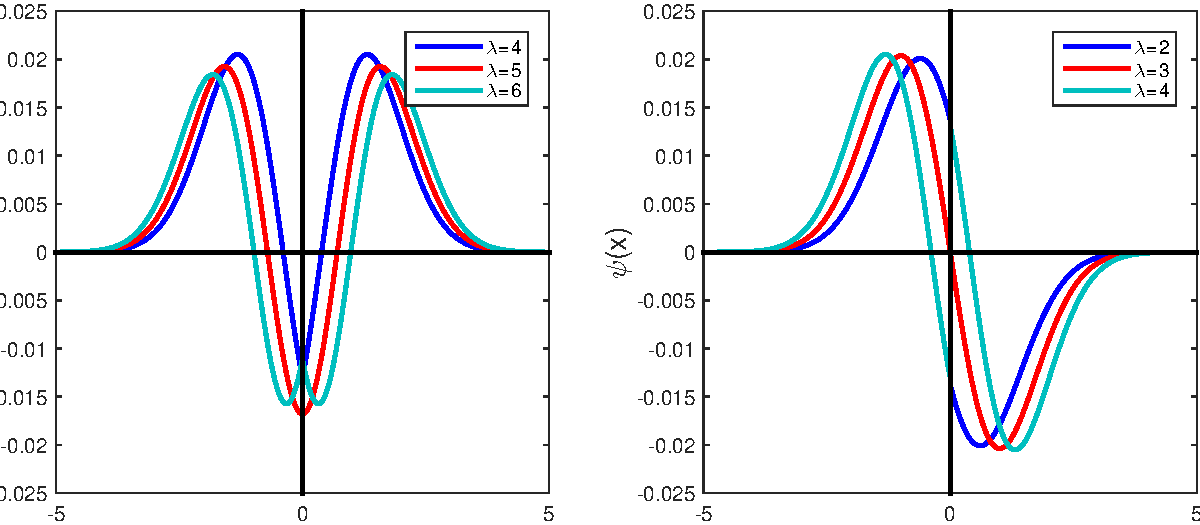
\includegraphics[width=4.5in]{07.ode3/qmho_mismatch.pdf}
   \caption{Wave functions of quantum harmonic oscillator. Left: Symmetric state. When the value of $\lambda$ is not right (blue and turquoise), the wave function is not smoothly connected at $x=0$.  When $\lambda$ is the correct eigenvalue, the curve is smooth everywhere.
      Right: Anti-symmetric state. Similarly to the symmetric function, when the value of $\lambda$ is not right (blue and turquoise), the wave function jumps at $x=0$.}
   \label{fig:qmho_mismatch}
\end{figure}


\subsection{Bouncing Quantum Particle}\label{sec:bounce_qm}


In Sec. 5.3.1, we discussed how to compute the wave function of a particle in a uniform gravity.
The particle keeps falling forever in that calculation.  Now, we put a floor so that the particle can bounce back.  We want to know what energy (eigenvalue) the particle can have and what is the corresponding eigenfunction.  We stat with the Schrodinger equation (5.11).  We set the reference of energy  so that the potential energy is zero at the floor ($y=0$). Using $\sqrt[3]{\displaystyle\frac{2m^2 g}{\hbar^2}}$ and $\sqrt[3]{\displaystyle\frac{m g^2 \hbar^2}{2}}$ as units for length and energy, the Schr\"{o}dinger equation is simplified to
\begin{equation}\label{eq:bounce_qm}
\left [ \frac{\md^2}{\md y^2}+ (E-y) \right ] \psi(y) = 0
\end{equation}
Since the particle cannot go below the floor, a boundary condition is $\psi(0)=0$.  The other boundary condition $\displaystyle\lim_{y \rightarrow \infty} \psi(y) = 0$ is replaced with $\psi(L)=)$ with a large value of $L$.

As we discussed in Sec 3.5.1, a solution to this equation is $\Ai (y-E)$. Applying the boundary condition at $y=0$, $\Ai(-E)=0$.  Therfore, the energy eigenvalues are $E_n=-z_n$ where $z_n$ is the $n$-th root of the airy function $\Ai(z_n)=0$. The first few roots of the airy function is listed in Table \ref{tbl:airy_roots}.

Now, we try to find the eigenvalue by solving the differential equation directly.  We integrate from  $y=L$ to $y=0$ by the Numerov method and use the secant method to find an eigenvalue. (Algorithm \ref{algo:eigen_shooting_secant})  The first five eigenvalues are listed in Table \ref{tbl:airy_roots}.  They are in a good agreement with the roots of the airy function.  As warned earlier in this chapter, the secant root finding not always find a root nearest to the initial guess.  Notice that the initial guess of the 5-th eigenvalues are below the 4-th eigenvalue.  

\begin{table}
\centering
\begin{tabular}{c|c|c|c}
\hline
n & root & initial guess & numerical eigenvalue\\
\hline
1 & -2.33811&2&2.3381074\\
2 & -4.08795&3&4.0879494\\
3 & -5.52056&5&5.5205605\\
4 & -6.78671&7&6.7867934\\
5 & -7.94413&6&7.9473771\\
\hline
\end{tabular}
\caption{The first five roots of airy function $\Ai(x)$ and eigenvalues by numerically solving the Schr\"{o}dinger equation (\ref{eq:bounce_qm}).}
\label{tbl:airy_roots}
\end{table}

\begin{figure}
\centering
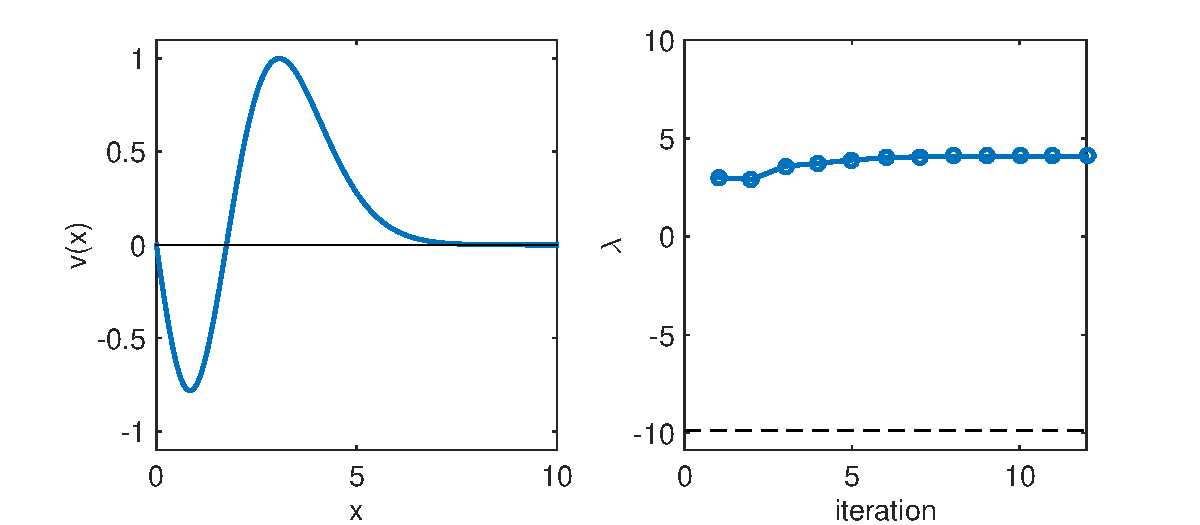
\includegraphics[width=5.5in]{07.ode3/bounce_qm.pdf}
\caption{Wavefuntions and eigenvalues of a quantum bouncing particle. Left: The energy eigenfunctions of the lowest three states.
Right: The levels of the three lowest energy eigenstates.}\label{fig:bounce_qm}
\end{figure}

\subsection{Diatomic Molecules}



The vibrational state of a diatomic molecule such as $H_2$ is described by a radial wave function $\psi(r)$. The wave function is determined by the energy eigenvalue equation
\begin{equation}\label{eq:qm_morse}
-\frac{\hbar^2}{2\mu} \frac{d^2 \psi}{dr^2} + \left[
U(r) + \frac{\hbar^2 \ell (\ell + 1)}{r} \right] \psi = \lambda \psi.
\end{equation}
where $\mu$. $\lambda$, and $\ell$ are reduced mass, energy eigenvalue, and angular quantum number, respectively.  The interaction potential is often approximated by the Morse potential
\begin{equation}
U(r) = D_e \left[
\me^{-2 \alpha (r-r_0)} - 2 \me^{-\alpha (r-r_0)} \right ]
\end{equation}
where $D_e$, $r_0$ and $\alpha$ are dissociation energy, equilibrium distance between the atoms and decay constant.  Their values for hydrogen and iodine molecules are listed in Table \ref{tbl:morse}.



When $\ell=0$, analytical solutions\footnote{Strictly speaking $\infty > r \ge 0$.  However, $\infty> r > -\infty$ is assumed.  This is a reasonable approximation since the potential diverges to $+\infty$ as $r$ goes to $-\infty$.} are known.\cite{qm_morse}  The eigenvalues are
\begin{equation}
\lambda_n = -D_e \left[ 1-\frac{\alpha \hbar}{\sqrt{2\mu D_e}}
\left( n+\frac{1}{2} \right) \right]^2 
\end{equation}
where $n$ is non-negative integer smaller than $\displaystyle\frac{\sqrt{2\mu D_e}}{\alpha\hbar} - \frac{1}{2}$.
The corresponding eigenfunctions are
\begin{equation}\label{eq:morse_exact}
\psi_n(r) = e^{-\xi/2} \xi^2  L_n^{(2s)} (\xi)
\end{equation}
where
\begin{equation}
\xi = \frac{2\sqrt{2\mu D_e}}{\alpha \hbar} \me^{-\alpha (r-r_0)} , \qquad
s = \frac{\sqrt{-2 \mu \lambda}}{\alpha \hbar}\,.
\end{equation}
and $L_n^{2s}$ is generalized Laguerre function which can be evaluated by the recursive equation
\begin{equation}
n L_n^{(a)} (x) = (2n - 1 + a - x) L_{n-1}^{(a)}(x)
+ (1 - a - n) L_{n-2}^{(a)} (x)
\end{equation}
with $L_0^{(a)}(x) = 1$ and $L_1^{(a)}(x)=1+a-x$.

Even when analytical solution is known, numerical analysis of the problem sometimes helps understanding the physics more quickly than analytical approach. Not many people can visualize hypergeometric functions in their head.


\begin{table}
	\caption{Values of the constants for the Morse potential.}
	\label{tbl:morse}
	\begin{center}
		\begin{tabular}{c|ccc}
			\hline
			Molecule&$r_0$(\AA)&$D_e$ (eV)& $\alpha r_0$ \\
			\hline
			\hline
			$H_2$&0.742&4.75&1.44\\
			$I_2$&2.66&1.56&4.94\\
			\hline
		\end{tabular}
	\end{center}
\end{table}

To implement a numerical method, we need some preparation.
The boundary condition $\displaystyle\lim_{x \rightarrow \infty} \psi(x)=0$ must be replaced by $\psi(x_\text{max}) = 0$ where $x_\text{max}$ is chosen such that $\psi(x_\text{max}) < \text{tolerance}$.  How can we find such a value?  The best way is to find a similar problem which can be solved analytically and find  $x_\text{max}$ usng the analytical solution.  The value for the original problem should be similar to that. For the present problem, the motion of the atoms should be close to a harmonic oscillation. Therefore, we consider a small amplitude approximation of the Morse potential.\cite{hooke}.  Expanding $U(r)$ in a Taylor series around the equilibrium position, we obtain a harmonic potential
\begin{equation}
U(r) \approx -D_e + D_e \alpha^2 (r-r_0)^2
\end{equation}
and the corresponding spring constant is $k=2 D_e \alpha^2$ or frequency $\omega = \sqrt{2 D_e \alpha^2 / \mu}$.  The ground state of the harmonic oscillator has wave function
\begin{equation}
u(x) \propto \me^{- x^2/2 a^2 }\, .
\end{equation}
where $a=\sqrt{\hbar/\mu \omega}$.
If we choose $x_\text{max} = 6 a$, the wave function at the boundary is $u(x_\text{max})/u(0) = \me^{-18}\sim 10^{-8}$ which is small enough.  This value should good enough at least for low energy states.

Program \ref{prog:morse} solves Eq. (\ref{eq:qm_morse})  for the lowest three eigenvalues using Algorithm \ref{algo:eigen_shooting_bisection}.   The results are
\begin{center}
\begin{minipage}{4in}
\small
\begin{Verbatim}[frame=single]
n=0, E=-0.1646901622, Exact=-0.1646901622
n=1, E=-0.1458135760, Exact=-0.1458135781
n=2, E=-0.1280854412, Exact=-0.1280856284
\end{Verbatim}
\normalsize
\end{minipage}
\end{center}
The agreement is very good.  However, the error increases as $n$ increases.  The error is due to the choice of $x_\text{max}$ which is supposed to be $\infty$.  Figures \ref{fig:morse} show the energy levels with respect to the potential energy profile (left panel) and eigen functions (right panel).


\begin{figure}
\centering
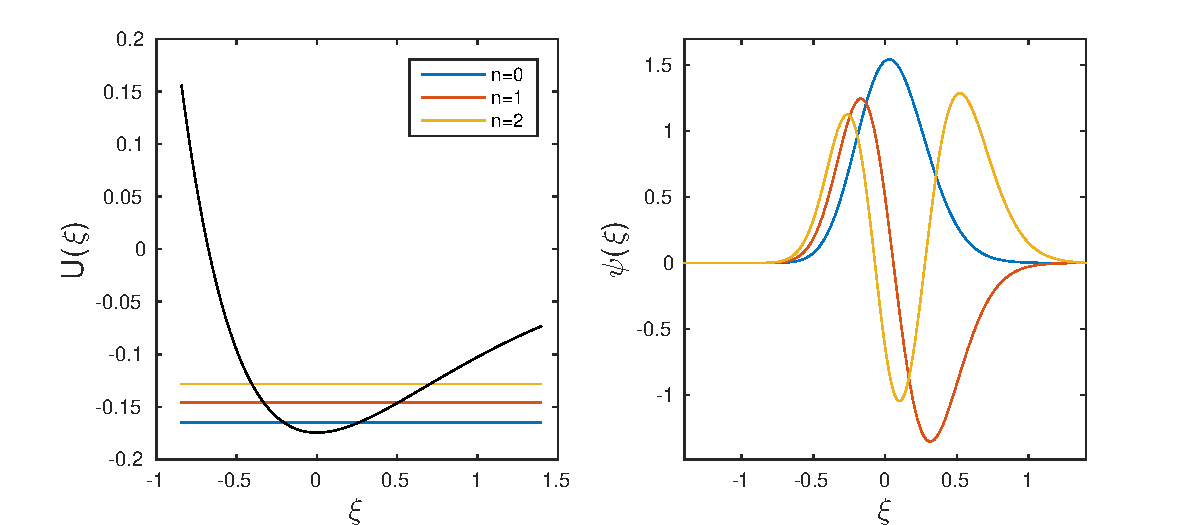
\includegraphics[width=5.5in]{07.ode3/morse.pdf}
\caption{Left: The Morse potential and the three lowest eigenvalues. Right: Wavefuntions corresponding toe the three eigenvalues shown in the left panel.}\label{fig:morse}
\end{figure}

\bigskip
\exercise
Compare the numerically obtained eigenfunctions  with the  analytical solution (\ref{eq:morse_exact}.


\vfill

\newpage
\noindent
\section{Problems}

\begin{enumerate}[labelwidth=0.5cm,labelindent=0cm,leftmargin=*,label=\bfseries \thechapter.\arabic*,align=left]

\item \textbf{Quantum Particle in a Square Potential} 

In Sec. 3.6.4, the energy of the particle in a square potential is evaluated numerically.  Here, we solve the Schr\"{o}dinger equation directly.  The potential energy (See Fig. 3.7) is given by
\begin{equation}
V(x) = \begin{cases}
0 & \text{for } |x|<a \\
V_0 & \text{for } |x|>a
\end{cases}
\end{equation}
Using $a$ and $\displaystyle\frac{\hbar^2}{2m a^2}$ as units of length and energy respectively,
the Schr\"{o}dinger equation is written as
\begin{equation}
\left [-\frac{\md^2}{\md x^2} + V(x) \right ] \psi(x) = E \psi(x)
\end{equation}

The parameter value $z_0=6$ in Sec 3.6.4 corresponds to $V_0=36$  [See Eq. (3.25b).].  The root finding program in Sec.3.6.4 found four energy eigenvalues, $E = z^2 =  1.81, 7.18, 15.89, 27.31$.
Modify the code used in Section \ref{sec:qmho_eigenvalue} (or write your own code in your favorite language) and find all four eigenvalues.  Compare the results with the results obtained in Sec.\ref{sec:quantum-well}

\item \textbf{Bound States in a Symmetric Potential}

A quantum particle of mass $m$ is bound in a potential
\begin{equation}
U(x) = - \frac{U_0}{\cosh^2 \alpha x}\, .
\end{equation}
Find all energy eigenvalues of the bound states.

Analytical solutions are given by
\begin{equation}
E_n = - \frac{\hbar^2 \alpha^2}{8 m} \left [ -(2n+1)+\sqrt{1+\frac{8 m U_0}{\hbar^2 \alpha^2}} \right ]
\end{equation}
and
\begin{equation}
\psi_n(x) = (1-\xi^2)^{\varepsilon/2} F[\varepsilon-s, \varepsilon+s+1,\varepsilon+1,(1-\xi)/2]
\end{equation}
where $F$ is the hypergeometric function and
\begin{equation}
\xi=\tanh \alpha x, \qquad \varepsilon = \frac{\sqrt{-2 m E_n}}{\hbar \alpha}, \qquad s=\frac{1}{2} \left ( -1+\sqrt{1+\frac{8 m U_0}{\hbar^2 \alpha^2}} \right )
\end{equation}

\end{enumerate}

\newpage
\section*{MATLAB Source Codes}
\addcontentsline{toc}{section}{\protect\numberline{}MATLAB Source Codes}


\bigskip
\noindent
\program
\label{prog:standing_wave}

\footnotesize
\begin{verbatim}
%**************************************************************************
%*     Example  7.1                                                       *
%*     filename: ch07pr01.m                                               *
%*     program listing number: 7.1                                        *
%*                                                                        *
%*     This program finds the first two eigen modes of standing wave in a *
%*     string using the shooting method (Numerov and secant methods).     *
%*                                                                        *
%*     Programmed by Ryoichi Kawai for Computational Physics Course.      *
%*     Last modification:  02/04/2017.                                    *
%**************************************************************************
clear all;

% setting the grid
xmin=0.0;
xmax=1.0;
N=200;
h=(xmax-xmin)/N;
x = linspace(xmin,xmax,N+1);
v=zeros(1,N+1);

% control parameters
tol=1e-6;
delta=1;
found=false;
kmax=100;


lambda(1) = 1;
k=1;

while not(found) & k<kmax
    
    % integrate ODE by Numerov method
    w = -lambda(k);
    v(1)=0;
    v(2)=delta;
    for n=2:N-1
        v(n+1) = 2*(1-5*h^2*w/12)*v(n) - (1+h^2*w/12)*v(n-1);
        v(n+1) = v(n+1)/(1+h^2*w/12);
    end
    
    % error in the boundary condition
    err(k) = v(N);
    
    if abs(err(k)) < tol
        found = true;
    else
        % secant method to guess next lambda
        if k == 1
            lambda(k+1) = lambda(k)-0.1;
        else
            lambda(k+1) = lambda(k) ...
                -(lambda(k)-lambda(k-1))/(err(k)-err(k-1))*err(k);
        end
        k=k+1;
    end
end
s=max(v);
v=v/s;
fprintf('lambda = %.7f, exact=%.7f\n',lambda(k),-pi^2);


subplot(1,2,1)
p=plot(x,v);
set(p,'linewidth',2)
xlabel('x','fontsize',14);
ylabel('v(x)','fontsize',14);
axis([ 0 1 -1.1 1.1]);
hold on

subplot(1,2,2)
r=plot([1:k],lambda(1:k),'-o');
set(r,'linewidth',2)
xlabel('iteration','fontsize',14)
ylabel(texlabel('lambda'),'fontsize',14)
axis([0 k -(2*pi)^2*1.1 10] )
hold on
r=plot([0,k],[-pi^2, -pi^2],'--');
set(r,'color','black')
hold on
r=plot([0,k],[-(2*pi)^2, -(2*pi)^2],'--');
set(r,'color','black')
hold on

found = false;
lambda(1) = -30;
k = 1;

while not(found)
    w = -lambda(k);
    v(1)=0;
    v(2)=delta;
    for n=2:N-1
        v(n+1) = 2*(1-5*h^2*w/12)*v(n) - (1+h^2*w/12)*v(n-1);
        v(n+1) = v(n+1)/(1+h^2*w/12);
    end
    err(k) = v(N);
    if abs(err(k)) < tol
        found = true;
    else
        if k == 1
            lambda(k+1) = lambda(k)-0.1;
        else
            lambda(k+1) = lambda(k) ...
                -(lambda(k)-lambda(k-1))/(err(k)-err(k-1))*err(k);
        end
        k=k+1;
    end
end
s = max(v);
v = v/s;
fprintf('lambda = %.7f, exact=%.7f\n',lambda(k),-(2*pi)^2);

subplot(1,2,1)
p=plot(x,v);
set(p,'linewidth',2,'color','red')
legend(texlabel('lambda_0=1'),texlabel('lambda_0=-30'));
legend('location','southwest');
r=plot([0,1],[0,0]);
set(r,'color','black')
hold off
subplot(1,2,2)
r=plot([1:k],lambda(1:k),'-o');
set(r,'linewidth',2,'color','red')
hold off
\end{verbatim}
\normalsize

\ruleend

\bigskip
\noindent
\program
\label{prog:qmho_eigenvalue}

\footnotesize
\begin{verbatim}
%**************************************************************************
%*     Section 7.2.1                                                      *
%*     filename: ch07pr02.m                                               *
%*     program listing number: 7.2                                        *
%*     Uses: qmho_numerov.m                                               *
%*                                                                        *
%*     This program finds an eigenvalue and eigenfunction of a quantum    *
%*     harmonic oscillator within a given bracket using the shooting      *
%*     method (Numerov and bisection methods).                            *
%*     Parity symmetry is taken into account.                             *
%*                                                                        *
%*     Programmed by Ryoichi Kawai for Computational Physics Course.      *
%*     Last modification:  10/13/2013.                                    *
%**************************************************************************
clear all;

E(1)=input('Energy Lower Blacket =');
E(2)=input('Energy Upper Blacket =');

symmetric = false;
anti_symmetric = false;
found = false;
xmax=5;
tol = 1e-8;
h = 0.001;

% Initial Lower bound
[x,psi] = qmho_numerov(E(1),xmax,h);
N=size(x,2);
error_L=(psi(N)-psi(N-1))/(x(N)-x(N-1));
error_L2=psi(N);
if abs(error_L) < tol
    found = true;
    symmetric = true;
    EM = E(1);
elseif abs(error_L2) < tol
    found = true;
    anti_symmeric = true;
    EM = E(1);
end

% Initial Upper bound
if not(found)   
   [x,psi] = qmho_numerov(E(2),xmax,h);
   error_U=(psi(N)-psi(N-1))/(x(N)-x(N-1));
   error_U2=psi(N);
   if abs(error_U) < tol
      found = true;
      symmetric = true;
      EM = E(2);
   elseif abs(error_U2) < tol
      found = true;
      anti_symmeric = true;
      EM = E(2);
   end
   if error_U*error_L<0
      symmetric = true;
   elseif error_U2*error_L2<0
      anti_symmetric = true;
      error_U = error_U2;
      error_L = error_L2;
   else
      error('Blacket error!');    
   end
   if symmetric & anti_symmetric
      error('Blacket error2!');
   end
end
    
% Begin bisection
while not(found)
    EM = sum(E)*0.5;
    [x,psi] = qmho_numerov(EM,xmax,h);
    if symmetric
        error_M=(psi(N)-psi(N-1))/(x(N)-x(N-1));
    else
        error_M=psi(N);
    end

    if abs(error_M)<tol
        found = true;
    else
        if error_M*error_L < 0
            E(2) = EM;
            error_U = error_M;
        else
            E(1) = EM;
            error_L = error_M;
        end
    end
end

% output the result
if symmetric
    fprintf('Symmetric state: ')
elseif anti_symmetric
    fprintf('Anti-Symmetric state: ')
end
fprintf('Eigenvalue= %.6f\n', EM);

X(1:N) = x(1:N);
X(N+1:2*N-1)=-x(N-1:-1:1);
if symmetric
    Y(1:N) = psi(1:N);
    Y(N+1:2*N-1)=psi(N-1:-1:1);
else
    Y(1:N) = psi(1:N);
    Y(N+1:2*N-1)=-psi(N-1:-1:1);
end

A = sum(Y(1:2:2*N-3).^2+4*Y(2:2:2*N-2).^2+Y(3:2:2*N-1).^2)*h/3;
Y = Y / sqrt(A);
p=plot(X,Y,[-xmax,xmax],[0,0],[0,0],[-1,1]);
set(p(1),'linewidth',2,'color','blue')
set(p(2:3),'color','black')
xlabel('x','fontsize',14)
ylabel(texlabel('psi(x)'),'fontsize',14)
\end{verbatim}

\begin{verbatim}
function [x,psi] = qmho_numerov(E,xmax,h)

W = @(x) -(x^2-E);

N=round(xmax/h);
xmax=h*N;
x = linspace(-xmax,0.0,N+1);
w = -x.^2+E;
psi = zeros(N+1);
psi(1)=0;
psi(2)=0.001;

% shoot out to x=0  by the Numerov method
  for n=2:N
    psi(n+1) = 2*(1-5*h^2*w(n)/12)*psi(n) - (1+h^2*w(n-1)/12)*psi(n-1);
    psi(n+1) = psi(n+1)/(1+h^2*w(n+1)/12);
  end
end
\end{verbatim}

\normalsize
\ruleend

\bigskip
\noindent
\program
\label{prog:bouncing_qm_ball}
\footnotesize
\begin{verbatim}
%**************************************************************************
%*     Section 7.2.2                                                      *
%*     filename: ch07pr03.m                                               *
%*     program listing number: 7.3                                        *
%*                                                                        *
%*     This program finds an eigenvalue and eigenfunction of a quantum    *
%*     bouncing ball within a given bracket using the shooting            *
%*     method (Numerov and secant methods).                               *
%*                                                                        *
%*     Programmed by Ryoichi Kawai for Computational Physics Course.      *
%*     Last modification:  02/04/2017.                                    *
%**************************************************************************
clear all;

% setting the grid
L=10; N=500; h=L/N;
x=linspace(0.0,L,N+1);
psi=zeros(N+1);

% control parameter
tol=1e-6;
delta = 0.01;
found = false;
kmax=100;


eigval(1) = input('Initial Guess =');  % initial guess

% secant iteration
k=1;
while not(found)
    % Numerov integration
    w = eigval(k)-x;
    psi(N+1)=0;
    psi(N)=delta;

    for n=N:-1:2
        psi(n-1) = 2*(1-5*h^2*w(n)/12)*psi(n) - (1+h^2*w(n+1)/12)*psi(n+1);
        psi(n-1) = psi(n-1)/(1+h^2*w(n-1)/12);
    end
    
    err(k) = psi(1);  % last point should be zero
    if abs(err(k)) < tol
        found = true;
    else
        if k == 1
            eigval(k+1) = eigval(k)-0.1;  % second guess
        else
            eigval(k+1) = eigval(k) ... % suggestion by the secant method
                -(eigval(k)-eigval(k-1))/(err(k)-err(k-1))*err(k);
        end
        k=k+1;
    end
end

% normalize the solution at the maximum
psi=psi/max(psi);
fprintf('lambda = %.7f\n',eigval(k));

% plot eigenfunction
subplot(1,2,1)
p=plot(x,psi);
set(p,'linewidth',2)
hold on
q=plot([x(1),x(N)],[0,0]);
set(q,'color','black')
xlabel('x','fontsize',14);
ylabel('v(x)','fontsize',14);
axis([ 0 L -1.1 1.1]);

% plot eigenvalue
subplot(1,2,2)
r=plot([1:k],eigval(1:k),'-o');
set(r,'linewidth',2)
xlabel('iteration','fontsize',14)
ylabel('E','fontsize',14)
axis([0 k -pi^2*1.1 10] )
hold on
r=plot([0,k],[-pi^2, -pi^2],'--');
set(r,'color','black')
hold off
\end{verbatim}
\normalsize

\ruleend

\bigskip
\noindent
\program
\label{prog:morse}
\footnotesize
\begin{verbatim}
%**************************************************************************
%*     Section 7.2.3                                                      *
%*     filename: ch07pr04.m                                               *
%*     program listing number: 7.4                                        *
%*                                                                        *
%*     This program finds an eigenvalue and eigenfunction of a quantum    *
%*     particle in the Morse potential using the shooting.                *
%*     method (Numerov and secant methods).                               *
%*                                                                        *
%*     Programmed by Ryoichi Kawai for Computational Physics Course.      *
%*     Last modification:  10/13/2013.                                    *
%**************************************************************************
clear all
clc

% Use the atomic unit
mp=1836.4;
e=27.2114;
a0=0.529177;
% parameters for H2
D=4.75/e; R0=0.742/a0; a=1.44/R0; name='H_2'; m=mp; mu=m/2;

% parameters for I2
%D=1.56/e; R0=2.66/a0; a=4.94/R0; name='I_2'; m=127*mp; mu=m/2;

% zero point energy
omega=sqrt(2*D*a^2/mu);
DE=omega/5;
d=1/sqrt(mu*omega)*12;


% define the discrete coordinate
N=1000;
h=d/N;
x=linspace(-d/2,d/2,N+1);
psi=zeros(1,N+1);
phi=zeros(3,N+1);
% evaluate the potential
U=D*(exp(-2*a*x)-2*exp(-a*x));

E_M=-D;

for L=1:3
% Initial Bracketting
E_L = E_M+DE;
w = 2*mu*(E_L-U);
psi(1)=0;
psi(2)=0.1;
% shoot out to x=L by the Numerov method
for n=2:N
   psi(n+1) = 2*(1-5*h^2*w(n)/12)*psi(n) - (1+h^2*w(n-1)/12)*psi(n-1);
   psi(n+1) = psi(n+1)/(1+h^2*w(n+1)/12);
end
ERR_L=psi(N+1);
found=false;

while not(found)
    E_U = E_L+DE;
    if E_U>0
        error
    end
    w = 2*mu*(E_U-U);
    psi(1)=0;
    psi(2)=0.1;
    for n=2:N
        psi(n+1) = 2*(1-5*h^2*w(n)/12)*psi(n) - (1+h^2*w(n-1)/12)*psi(n-1);
        psi(n+1) = psi(n+1)/(1+h^2*w(n+1)/12);
    end
    ERR_U=psi(N+1);
    if ERR_L*ERR_U<0
        found=true;
    else
        E_L=E_U;
        ERR_L=ERR_U;
    end
end

found=false;
tol1=1e-8;
tol2=1e-15;

while not(found)
    E_M=(E_L+E_U)/2;
    w = 2*mu*(E_M-U);
    psi(1)=0;
    psi(2)=0.1;
 
    for n=2:N
        psi(n+1) = 2*(1-5*h^2*w(n)/12)*psi(n) - (1+h^2*w(n-1)/12)*psi(n-1);
        psi(n+1) = psi(n+1)/(1+h^2*w(n+1)/12);
    end
    ERR_M=psi(N+1);
    if abs(ERR_M) < tol1 || abs(E_L-E_M)<tol2
        found = true;
    end
    
    if ERR_M*ERR_L > 0 
        E_L=E_M;
    else
        E_U=E_M;
    end

end
  eigval(L) = E_M;
  % normalize the wave function
  z=sum(psi.^2)*h;
  phi(L,:)=psi/sqrt(z);
  exact=-D*(1-a/sqrt(2*mu*D)*(L-1/2))^2;
  fprintf('n=%d, E=%.10f, Exact=%.10f\n',L-1,E_M,exact)
end


% Ploting potential and eigenvalues
subplot(1,2,1)
N0=ceil(N/5);
p=plot([x(N0),x(N)],[eigval(1),eigval(1)],...
       [x(N0),x(N)],[eigval(2),eigval(2)],...
       [x(N0),x(N)],[eigval(3),eigval(3)]);
legend(p,'n=0','n=1','n=2')
hold on
plot(x(N0:N),U(N0:N),'color','black')
hold off
xlabel(texlabel('xi'),'fontsize',14)
ylabel(texlabel('U(xi)'),'fontsize',14)

% Ploting wave functions
subplot(1,2,2)
plot(x,phi(1,:),x,phi(2,:),x,phi(3,:))
ymax=max(phi(:));
ymin=min(phi(:));
axis([-d/2 d/2 ymin*1.1 ymax*1.1])
xlabel(texlabel('xi'),'fontsize',14)
ylabel(texlabel('psi(xi)'),'fontsize',14)
\end{verbatim}
\normalsize

\ruleend

\bigskip
\noindent
\section*{Python Source Codes}
\addcontentsline{toc}{section}{\protect\numberline{}Python Source Codes}
\setcounter{program}{0}

\bigskip
\noindent
\program
\footnotesize
\begin{verbatim}
#!/usr/bin/env python3
# -*- coding: utf-8 -*-
"""
%**************************************************************************
%*     Example  7.1                                                       *
%*     filename: ch07pr01.py                                              *
%*     program listing number: 7.1                                        *
%*                                                                        *
%*     This program finds the first two eigen modes of standing wave in a *
%*     string using the shooting method (Numerov and secant methods).     *
%*                                                                        *
%*     Programmed by Ryoichi Kawai for Computational Physics Course.      *
%*     Last modification:  02/04/2017.                                    *
%**************************************************************************
"""
import numpy as np
import matplotlib.pyplot as plt

# setting the grid
xmin=0.0
xmax=1.0
N=200
h=(xmax-xmin)/np.float(N)
x=np.linspace(xmin,xmax,N+1)
v = np.zeros(N+1)

# control parameter
kmax=100
tol=1.0e-6
delta = 1.0
found = False

lam=np.zeros(kmax+1)
err=np.zeros(kmax+1)
lam[0] = 1.0

k=0
while not(found) and k < kmax:
    
    # integrate ODE by Numerov method
    w = -lam[k]
    v[0]=0.0
    v[1]=delta
    for n in range(1,N):
        v[n+1] = 2.0*(1.0-5.0*h**2*w/12.0)*v[n] - (1.0+h**2*w/12.0)*v[n-1]
        v[n+1] = v[n+1]/(1.0+h**2*w/12.0)

    
    # error in the boundary condition
    err[k] = v[N]
    
    if np.abs(err[k]) < tol:
        found = True
    else:
        # secant method to guess next lambda
        if k == 0:
            lam[k+1] = lam[k]-0.1
        else:
            lam[k+1] = lam[k]-(lam[k]-lam[k-1])/(err[k]-err[k-1])*err[k]
        k+=1

s=max(v)
v=v/s
print('lambda = {0:12.7f}, exact={1:12.7f}'.format(lam[k],-np.pi**2))

plt.figure(figsize=(12,5))
plt.subplot(1,2,1)
plt.plot(x,v,'-b',label=r"\lambda_0=1$")
plt.xlabel('x',fontsize=14)
plt.ylabel('v(x)',fontsize=14)

plt.subplot(1,2,2)
plt.plot(np.linspace(0,k,k+1),lam[0:k+1],'-ob')
plt.plot([0,k],[-np.pi**2, -np.pi**2],'--k')
plt.plot([0,k],[-(2*np.pi)**2, -(2*np.pi)**2],'--k')
plt.xlabel('iteration',fontsize=14)
plt.ylabel(r'$\lambda$',fontsize=14)


found = False

lam[0]= -30

k=0
while not(found) and k < kmax:
    w = -lam[k]
    v[0]=0.0
    v[1]=delta
    for n in range(1,N):
        v[n+1] = 2.0*(1.0-5.0*h**2*w/12.0)*v[n] - (1.0+h**2*w/12.0)*v[n-1]
        v[n+1] = v[n+1]/(1.0+h**2*w/12.0)

    err[k] = v[N]
    if abs(err[k]) < tol:
        found = True
    else:
        if k == 0:
            lam[k+1] = lam[k]-0.1
        else:
            lam[k+1] = lam[k] -(lam[k]-lam[k-1])/(err[k]-err[k-1])*err[k]

        k+=1


s = max(v)
v = v/s
print('lambda = {0:12.7f}, exact={1:12.7f}'.format(lam[k],-(2*np.pi)**2))

plt.subplot(1,2,1)
plt.plot(x,v,'-r',label=r"\lambda_0=-30$")
plt.legend(loc=3)

plt.subplot(1,2,2)
plt.plot(np.linspace(0,k,k+1),lam[0:k+1],'-or')

plt.show()
\end{verbatim}
\normalsize

\ruleend

\bigskip
\noindent
\program
\footnotesize
\begin{verbatim}
#!/usr/bin/env python3
# -*- coding: utf-8 -*-
"""
%**************************************************************************
%*     Section 7.2.1                                                      *
%*     filename: ch07pr02.py                                              *
%*     program listing number: 7.2                                        *
%*                                                                        *
%*     This program finds an eigenvalue and eigenfunction of a quantum    *
%*     harmonic oscillator within a given bracket using the shooting      *
%*     method (Numerov and bisection methods).                            *
%*     Parity symmetry is taken into account.                             *
%*                                                                        *
%*     Programmed by Ryoichi Kawai for Computational Physics Course.      *
%*     Last modification:  02/04/2017.                                    *
%**************************************************************************
"""
import numpy as np
import matplotlib.pyplot as plt
import sys

def qmho_numerov(E,xmax,h):
    N=round(xmax/h)
    xmax = h*N
    psi=np.zeros(N+1)
    x =np.linspace(-xmax,0.0,N+1)
    w = -x**2+E

    psi[0]=0
    psi[1]=0.001

    # shoot out to x=L by the Numerov method
    for n in range(1,N):
        psi[n+1] = 2.0*(1.0-5.0*h**2*w[n]/12.0)*psi[n] \
            - (1.0+h**2*w[n-1]/12.0)*psi[n-1]
        psi[n+1] = psi[n+1]/(1+h**2*w[n+1]/12.0)

    return [x,psi]

if __name__ == "__main__":
    
    E=np.zeros(2)
    E[0]=np.float(input('Energy Lower Blacket ='))
    E[1]=np.float(input('Energy Upper Blacket ='))

    # control parameter
    symmetric = False;
    anti_symmetric = False
    found = False
    xmin=0.0
    xmax=5.0
    tol = 1e-8
    h = 0.001

    # Initial Lower bound
    [x,psi] = qmho_numerov(E[0],xmax,h)
    N=x.size-1
    error_L=(psi[N]-psi[N-1])/(x[N]-x[N-1])
    error_L2=psi[N]
    if np.abs(error_L) < tol:
        found = True
        symmetric = True
        EM = E[0]
    elif np.abs(error_L2) < tol:
        found = True
        anti_symmeric = True
        EM = E[0]

    # Initial Upper bound
    if not(found):   
        [x,psi] = qmho_numerov(E[1],xmax,h)
        error_U=(psi[N]-psi[N-1])/(x[N]-x[N-1])
        error_U2=psi[N]

        if np.abs(error_U) < tol:
            found = True
            symmetric = True
            EM = E[1]
        elif np.abs(error_U2) < tol:
            found = True
            anti_symmeric = True
            EM = E[1]

        if error_U*error_L<0:
            symmetric = True
        elif error_U2*error_L2<0:
            anti_symmetric = True
            error_U = error_U2
            error_L = error_L2
        else:
            sys.exit('Blacket error!');   

        if symmetric & anti_symmetric:
            sys.exit('Blacket error2!')
    
    # Begin bisection
    while not(found):
        EM = E.sum()*0.5
        [x,psi] = qmho_numerov(EM,xmax,h)
        if symmetric:
            error_M=(psi[N]-psi[N-1])/(x[N]-x[N-1])
        else:
            error_M=psi[N]

        if np.abs(error_M)<tol:
            found = True
        else:
            if error_M*error_L < 0:
                E[1] = EM
                error_U = error_M
            else:
                E[0] = EM
                error_L = error_M

    # output the result
    if symmetric:
        print('Symmetric state: ')
    elif anti_symmetric:
        print('Anti-Symmetric state: ')

    print('Eigenvalue= {0:12.6f}'.format(EM))

    X=np.zeros(2*N+1)
    Y=np.zeros(2*N+1)
    X[0:N+1] = x[0:N+1]
    X[N+1:2*N]=-x[N-1:0:-1]
    if symmetric:
        Y[0:N+1] = psi[0:N+1];
        Y[N+1:2*N]=psi[N-1:0:-1]
    else:
        Y[1:N] = psi[1:N]
        Y[N+1:2*N]=-psi[N-1:0:-1]

    A = sum(Y[0:2*N-3:2]**2+4.0*Y[1:2*N-2:2]**2+Y[2:2*N-1:2]**2)*h/3.0
    Y = Y / np.sqrt(A)
    plt.figure(figsize=(6,5))
    plt.plot(X,Y,'-b')
    plt.plot([-xmax,xmax],[0,0],'-k')
    plt.plot([0,0],[-1,1],'-k')
    plt.xlabel('x')
    plt.ylabel(r'$\psi(x)$')
    plt.show()
\end{verbatim}
\normalsize

\ruleend

\bigskip
\noindent
\program
\footnotesize
\begin{verbatim}
#!/usr/bin/env python3
# -*- coding: utf-8 -*-
"""
%**************************************************************************
%*     Section 7.2.2                                                      *
%*     filename: ch07pr03.py                                              *
%*     program listing number: 7.3                                        *
%*                                                                        *
%*     This program finds an eigenvalue and eigenfunction of a quantum    *
%*     bouncing ball within a given bracket using the shooting            *
%*     method (Numerov and secant methods).                               *
%*                                                                        *
%*     Programmed by Ryoichi Kawai for Computational Physics Course.      *
%*     Last modification:  02/04/2017.                                    *
%**************************************************************************
"""
import numpy as np
import matplotlib.pyplot as plt

# setting the grid
L=10.0; N=500; h=L/N
x=np.linspace(0,L,N+1)
psi=np.zeros(N+1)

# control parameter
tol=1e-6
delta = 0.01
found = False
kmax=100
eigval=np.zeros(kmax+1)
err=np.zeros(kmax+1)
eigval[0] = np.float(input('Initial Guess ='))  # initial guess

k=0
# secant iteration
while not(found) and k<kmax:
    # Numerov integration
    w = eigval[k]-x
    psi[N]=0.0
    psi[N-1]=delta
    for n in range(N-1,0,-1):
        psi[n-1]=2.0*(1.0-5.0*h**2*w[n]/12.0)*psi[n] \
            - (1.0+h**2*w[n+1]/12.)*psi[n+1]
        psi[n-1] = psi[n-1]/(1.0+h**2*w[n-1]/12.0)
    
    err[k] = psi[0] 
    if np.abs(err[k]) < tol:
        found = True
    else:
        if k == 0:
            eigval[k+1] = eigval[k]-0.1  # second guess
        else:
            # suggestion by the secant method
            eigval[k+1] = eigval[k] \
                -(eigval[k]-eigval[k-1])/(err[k]-err[k-1])*err[k]

        k+=1

# normalize the solution at the maximum
psi=psi/max(psi)
print('Eigenvalue = {0:12.7f}'.format(eigval[k]))

# plot eigenfunction
plt.figure(figsize=(12,5))
plt.subplot(1,2,1)
plt.plot(x,psi,'-b',linewidth=2)
plt.plot([x[0],x[N]],[0,0],'-k')
plt.xlabel('x',fontsize=14)
plt.ylabel('v(x)',fontsize=14)

# plot eigenvalue
plt.subplot(1,2,2)
plt.plot(np.linspace(0,k,k+1),eigval[0:k+1],'-ob')
plt.plot([0,k],[-np.pi**2, -np.pi**2],'--k');
plt.xlabel('iteration',fontsize=14)
plt.ylabel('E',fontsize=14)

plt.show()
\end{verbatim}
\normalsize

\ruleend

\bigskip
\noindent
\program
\footnotesize
\begin{verbatim}
#!/usr/bin/env python3
# -*- coding: utf-8 -*-
"""
%**************************************************************************
%*     Section 7.2.3                                                      *
%*     filename: ch07pr04.py                                              *
%*     program listing number: 7.4                                        *
%*                                                                        *
%*     This program finds an eigenvalue and eigenfunction of a quantum    *
%*     particle in the Morse potential using the shooting.                *
%*     method (Numerov and secant methods).                               *
%*                                                                        *
%*     Programmed by Ryoichi Kawai for Computational Physics Course.      *
%*     Last modification:  02/04/2017.                                    *
%**************************************************************************
"""
import numpy as np
import matplotlib.pyplot as plt
import sys


# Use the atomic unit
mp=1836.4
e=27.2114
a0=0.529177
# parameters for H2
D=4.75/e; R0=0.742/a0; a=1.44/R0; name='H_2'; m=mp; mu=m/2.

# parameters for I2
#D=1.56/e; R0=2.66/a0; a=4.94/R0; name='I_2'; m=127*mp; mu=m/2;

# zero point energy
omega=np.sqrt(2.0*D*a**2/mu)
DE=omega/5.0
d=1.0/np.sqrt(mu*omega)*12.0


# define the discrete coordinate
N=1000
h=d/N
x=np.linspace(-d/2.0,d/2.0,N+1)
psi=np.zeros(N+1)
phi=np.zeros((3,N+1))
# evaluate the potential
U=D*(np.exp(-2.0*a*x)-2.0*np.exp(-a*x))


eigval=np.zeros(3)
E_M=-D

for L in [0, 1, 2]:

    # Initial Bracketting
    E_L = E_M+DE
    w = 2*mu*(E_L-U)
    psi[0]=0.0
    psi[1]=0.1
    # shoot out to x=L by the Numerov method
    for n in range(1,N):
        psi[n+1] = 2.0*(1.0-5.0*h**2*w[n]/12.0)*psi[n] \
            - (1.0+h**2*w[n-1]/12.0)*psi[n-1]
        psi[n+1] = psi[n+1]/(1+h**2*w[n+1]/12.0)

    ERR_L=psi[N]
    found=False

    while not(found):

        E_U = E_L+DE
        if E_U>0.0:
            sys.exit('Blacket error')
            
        w = 2.0*mu*(E_U-U)
        psi[0]=0.0
        psi[1]=0.1
        for n in range(1,N):
            psi[n+1] = 2.0*(1.0-5.0*h**2*w[n]/12.0)*psi[n] \
                - (1.0+h**2*w[n-1]/12.0)*psi[n-1]
            psi[n+1] = psi[n+1]/(1+h**2*w[n+1]/12.0)

        ERR_U=psi[N]
        if np.sign(ERR_L)*np.sign(ERR_U)<0.0:
            found=True
        else:
            E_L=E_U
            ERR_L=ERR_U

    found=False
    tol1=1e-8
    tol2=1e-15

    while not(found):
        E_M=(E_L+E_U)/2.0
        w = 2.0*mu*(E_M-U)
        psi[0]=0.0
        psi[1]=0.1
 
        for n in range(1,N):
            psi[n+1] = 2.0*(1.0-5.0*h**2*w[n]/12.0)*psi[n] \
                - (1.0+h**2*w[n-1]/12.0)*psi[n-1]
            psi[n+1] = psi[n+1]/(1+h**2*w[n+1]/12.0)

        ERR_M=psi[N]
        if np.abs(ERR_M) < tol1 or np.abs(E_L-E_M)<tol2:
            found = True
    
        if np.sign(ERR_M)*np.sign(ERR_L) > 0.0 :
            E_L=E_M
        else:
            E_U=E_M

    eigval[L] = E_M
    # normalize the wave function
    z=sum(psi**2)*h
    phi[L,:]=psi/np.sqrt(z);
    exact=-D*(1.0-a/np.sqrt(2.0*mu*D)*(L+1./2.))**2
    print('n={0:3d}, E={1:10.7f}, Exact={2:10.7f}'.format(L-1,E_M,exact))


# Ploting potential and eigenvalues
plt.figure(figsize=(12,5))
plt.subplot(1,2,1)
N0=np.int(np.ceil(N/5))
plt.plot([x[N0],x[N]],[eigval[0],eigval[0]],'-b',label='n=0')
plt.plot([x[N0],x[N]],[eigval[1],eigval[1]],'-g',label='n=1')
plt.plot([x[N0],x[N]],[eigval[2],eigval[2]],'-r',label='n=2')
plt.plot(x[N0:N],U[N0:N],'-k')
plt.xlabel(r'$\xi$',fontsize=14)
plt.ylabel(r'$U(\xi)$',fontsize=14)
plt.legend(loc=1)

# Ploting wave functions
plt.subplot(1,2,2)
plt.plot(x,phi[0,:],'-b')
plt.plot(x,phi[1,:],'-g')
plt.plot(x,phi[2,:],'-r')
plt.xlabel(r'$\xi$',fontsize=14)
plt.ylabel(r'$\psi(\xi)$',fontsize=14)

plt.show()
\end{verbatim}

\normalsize

\ruleend

\newpage
%\chapbibliography
\bibliographystyle{unsrt}
\bibliography{compphys}